% ============================================================================
%  OhMyGAD — Student and Faculty User Manual
%  LaTeX Template
% ============================================================================
\documentclass[12pt, a4paper]{article}

% ── Packages ────────────────────────────────────────────────────────────────
\usepackage[utf8]{inputenc}
\usepackage[T1]{fontenc}
\usepackage{lmodern}
\usepackage[margin=1in]{geometry}
\usepackage{graphicx}
\graphicspath{{./}{student-faculty/}}
\usepackage[table]{xcolor}
\usepackage{hyperref}
\usepackage{booktabs}
\usepackage{longtable}
\usepackage{enumitem}
\usepackage{fancyhdr}
\usepackage{titlesec}
\usepackage{tocloft}
\usepackage{float}
\usepackage{caption}
\usepackage{parskip}
\usepackage{tabularx}
\usepackage{array}
\usepackage{microtype}
\usepackage{amssymb}

% ── Colours ─────────────────────────────────────────────────────────────────
\definecolor{primarydark}{HTML}{2D2A4A}
\definecolor{periwinkle}{HTML}{B8B5E8}
\definecolor{softpink}{HTML}{F4A7B9}
\definecolor{accentgold}{HTML}{F4C97A}
\definecolor{linkblue}{HTML}{2563EB}
\definecolor{lightgray}{HTML}{F5F5F5}

% ── Hyperlink styling ──────────────────────────────────────────────────────
\hypersetup{
  colorlinks  = true,
  linkcolor   = primarydark,
  urlcolor    = linkblue,
  citecolor   = primarydark,
  pdfauthor   = {OhMyGAD Development Team},
  pdftitle    = {OhMyGAD Student and Faculty User Manual},
  pdfsubject  = {User Manual for Student and Faculty Users},
}

% ── Header / Footer ───────────────────────────────────────────────────────
\pagestyle{fancy}
\fancyhf{}
\fancyhead[L]{\small\textcolor{primarydark}{OhMyGAD — Student and Faculty User Manual}}
\fancyhead[R]{\small\textcolor{primarydark}{\thepage}}
% \fancyfoot[C]{\small\textcolor{gray}{Confidential — For Internal Use Only}}
\renewcommand{\headrulewidth}{0.4pt}
\renewcommand{\footrulewidth}{0.2pt}

% ── Section styling ────────────────────────────────────────────────────────
\titleformat{\section}
  {\Large\bfseries\color{primarydark}}{\thesection}{1em}{}
\titleformat{\subsection}
  {\large\bfseries\color{primarydark}}{\thesubsection}{1em}{}
\titleformat{\subsubsection}
  {\normalsize\bfseries\color{primarydark}}{\thesubsubsection}{1em}{}

% ── Reusable screenshot placeholder ───────────────────────────────────────
\newcommand{\screenshotplaceholder}[1]{%
  \begin{figure}[H]
    \centering
    \fbox{\parbox{0.85\textwidth}{\vspace{4cm}
      \centering\textcolor{gray}{\textit{Screenshot: #1}}
    \vspace{4cm}}}
    \caption{#1}
  \end{figure}
}

\newcommand{\screenshotfigure}[3][0.95\textwidth]{%
  \begin{figure}[H]
    \centering
    \includegraphics[width=#1]{#2}
    \caption{#3}
  \end{figure}
}

% ── Reusable field-description table ──────────────────────────────────────
\newenvironment{fieldtable}{%
  \begin{longtable}{|>{\raggedright\arraybackslash}p{2.2cm}|>{\centering\arraybackslash}p{1.8cm}|>{\raggedright\arraybackslash}p{2.2cm}|>{\raggedright\arraybackslash}p{7.3cm}|}
  \hline
  \rowcolor{lightgray}
  \textbf{Field} & \textbf{Required} & \textbf{Limit} & \textbf{Validation \& Notes} \\
  \hline
  \endfirsthead
  \hline
  \rowcolor{lightgray}
  \textbf{Field} & \textbf{Required} & \textbf{Limit} & \textbf{Validation \& Notes} \\
  \hline
  \endhead
  \hline
  \endfoot
}{%
  \end{longtable}
}
\newcommand{\fieldrow}[4]{%
  #1 & #2 & #3 & #4 \\ \hline
}

% ════════════════════════════════════════════════════════════════════════════
\begin{document}

% ── Title Page ─────────────────────────────────────────────────────────────
\begin{titlepage}
  \centering
  \vspace*{3cm}

  {\Huge\bfseries\textcolor{primarydark}{OhMyGAD!}}\\[0.4cm]
  {\LARGE\textcolor{primarydark}{Student and Faculty User Manual}}\\[1.5cm]

  {\large Kasarian Gender Studies Program}\\[0.5cm]
  {\large University of the Philippines Baguio}\\[2cm]

  \textcolor{gray}{\today}\\[0.5cm]
  \textcolor{gray}{Version 1.0}

  \vfill
  {\small CMSC 128: Software Engineering}\\
  {\small by 128 Sheeps}
\end{titlepage}

% ── Table of Contents ──────────────────────────────────────────────────────
\tableofcontents
\newpage

% ════════════════════════════════════════════════════════════════════════════
%  1. INTRODUCTION
% ════════════════════════════════════════════════════════════════════════════
\section{Introduction}

\subsection{What is OhMyGAD?}
OhMyGAD is a web-based information system built for the \textbf{Kasarian Gender Studies Program} office of the University of the Philippines Baguio. It serves as a centralized platform where students and faculty can discover and register for GAD-related events, answer post-event surveys, read gender and development guidelines, and track their event attendance, all in one place.

\subsection{Who Is This Manual For?}
This manual is written for users who have been given the \textbf{Student} or \textbf{Faculty} role. These users can view events and register for them, answer surveys linked to events they have attended, read GAD guidelines, and update their own profile information.

\subsection{How to Use This Manual}
\begin{itemize}[leftmargin=1.5em]
  \item Each section covers one major page or feature of the system.
  \item \textbf{Screenshots} are provided to help you identify what you see on screen.
  \item \textbf{Field tables} list every input you can fill in, along with character limits and validation requirements.
  \item Fields marked with an asterisk (\textbf{*}) are required. The form will not submit without them.
\end{itemize}

\subsection{Accessing the System}
\begin{enumerate}[leftmargin=1.5em]
  \item Open your web browser (Chrome, Firefox, or Edge recommended).
  \item Navigate to this link: \url{https://upb-kasarian-omg.vercel.app/}
\end{enumerate}

\subsubsection*{If you do not have an account yet}
\begin{enumerate}[leftmargin=1.5em]
  \item On the Login page, click \textbf{Sign up} to go to the Sign Up page.
  \item Fill in your \textbf{Full Name}, \textbf{UP Mail}, \textbf{Password}, and \textbf{Repeat Password}, then click \textbf{Sign up}. Alternatively, click \textbf{Sign up with UP Mail} to register using your UP Mail directly.
  \item Complete the \textbf{onboarding process} by filling in your personal, academic, and identity information.
  \item After completing onboarding, you will be taken to your \textbf{Dashboard}.
\end{enumerate}

\subsubsection*{If you already have an account}
\begin{enumerate}[leftmargin=1.5em]
  \item Enter your \textbf{UP Mail} and \textbf{Password}, then click \textbf{Login}. Alternatively, click \textbf{Sign in with UP Mail} to log in using your Google account.
  \item You will be taken directly to your \textbf{Dashboard}.
\end{enumerate}

\screenshotfigure[0.75\textwidth]{sf-figures/1-Introduction/signup.png}{Sign Up Page}
\screenshotfigure[0.75\textwidth]{sf-figures/1-Introduction/login.png}{Login Page}
\screenshotfigure[0.75\textwidth]{sf-figures/1-Introduction/onboarding.png}{Onboarding Form}

% ════════════════════════════════════════════════════════════════════════════
%  2. DASHBOARD
% ════════════════════════════════════════════════════════════════════════════
\newpage
\section{Dashboard}

After logging in (and completing onboarding), you will land on your personal \textbf{Dashboard}. This page gives you a quick overview of your activity and upcoming events.

\subsection{Events Panel}
The centre of the dashboard shows a summary of events you have registered for, organized into three groups:

\begin{itemize}[leftmargin=1.5em]
  \item \textbf{Today} — Events that are happening today. These appear at the top so you never miss one.
  \item \textbf{Upcoming} — Events you have registered for that have not started yet, shown in chronological order by default.
  \item \textbf{Past} — Events you were registered for that have already ended.
\end{itemize}

Each event entry shows the event title, date, time, and location. Click an event to see its full details.

\subsection{Right Sidebar}
On the right side of the dashboard you will find a summary card showing your participation progress and pending tasks:

\begin{itemize}[leftmargin=1.5em]
  \item \textbf{GSO Sessions Attended} — How many Gender Sensitivity Orientation sessions you have attended, shown as a circular progress bar out of the required number.
  \item \textbf{ASHO Sessions Attended} — How many Anti-Sexual Harassment Orientation sessions you have attended, shown as a circular progress bar.
  \item \textbf{Pending Surveys} — A list of surveys linked to events you have attended that you have not yet answered.
\end{itemize}

\screenshotfigure[0.75\textwidth]{sf-figures/2-Dashboard/student-faculty-dashboard.jpg}{Student / Faculty Dashboard — Overview}

\subsection{Global Search}
At the top of every page you will find the \textbf{Search bar}. You can use it to quickly find events, guidelines, or surveys by typing a keyword. Results appear in a dropdown as you type.

\begin{fieldtable}
  \fieldrow{Search query}{No}{64 chars}{Type at least 2 characters to see results. Press \textbf{Enter} to open the full search results page. Click any result to navigate directly to that item.}
\end{fieldtable}

\screenshotfigure[0.75\textwidth]{sf-figures/2-Dashboard/dashboard-figure4-global_search.png}{Global Search — Dropdown Results}

% ════════════════════════════════════════════════════════════════════════════
%  3. EVENTS PAGE
% ════════════════════════════════════════════════════════════════════════════
\newpage
\section{Events Page}

The \textbf{Events} page shows all GAD-related events — orientations, forums, research sessions, training, and workshops. This is where you can browse events and register for ones you want to attend.

\subsection{Browsing Events}
Events are displayed as cards in a grid. Each card shows:
\begin{itemize}[leftmargin=1.5em]
  \item The event \textbf{title}
  \item The event \textbf{category}
  \item The event \textbf{open and close date and time}
  \item The event \textbf{registration open and close date and time}
  \item A \textbf{capacity bar} showing how many spots are filled
  \item A \textbf{status badge} (Upcoming, Today, or Past)
  \item If you are already registered, a \textbf{``Registered''} label appears on the button
\end{itemize}

\screenshotfigure[0.75\textwidth]{sf-figures/3-Events/today.png}{Dashboard — Discover Events Page (Today Tab)}
\screenshotfigure[0.75\textwidth]{sf-figures/3-Events/upcoming.png}{Dashboard — Discover Events Page (Upcoming Tab)}
\screenshotfigure[0.75\textwidth]{sf-figures/3-Events/past.png}{Dashboard — Discover Events Page (Past Tab)}

You can narrow down the list using the tools at the top of the page:

\begin{fieldtable}
  \fieldrow{Search}{No}{---}{Type any keyword to filter events by title, category, or location.}
  \fieldrow{Sort}{No}{Dropdown}{Sort events by title, category, status, date, capacity, or location.}
  \fieldrow{Filter}{No}{Dropdown}{Filter events by status (Today, Upcoming, Past) using the filter tabs, or by category using the dropdown. Multiple filters can be active at the same time. Active filters are shown as coloured chips below the toolbar.}
  \fieldrow{Status Tabs}{No}{Single-select}{Filter events by status (Today, Upcoming, or Past) by navigating through the tabs.}
\end{fieldtable}

\screenshotfigure[1\textwidth]{sf-figures/3-Events/search-sort-filter.png}{Events Page — Search, Sort, Filter, and Tab Controls}
\begin{figure}[H]
  \centering
  \begin{minipage}[b]{0.45\textwidth}
    \centering
    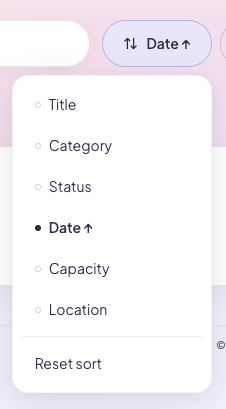
\includegraphics[width=0.45\textwidth]{sf-figures/3-Events/event-sort.png}
    \caption{Events Page — Sort Options}
  \end{minipage}\hfill
  \begin{minipage}[b]{0.45\textwidth}
    \centering
    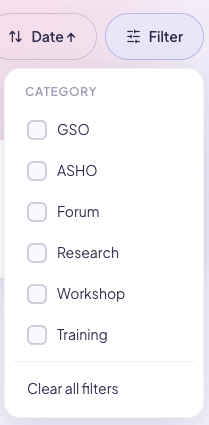
\includegraphics[width=0.45\textwidth]{sf-figures/3-Events/event-filter.png}
    \caption{Events Page — Filter Options}
  \end{minipage}
\end{figure}

\subsection{Viewing Event Details}
Click on any event card to open its \textbf{detail modal}. The modal shows:
\begin{itemize}[leftmargin=1.5em]
  \item A banner image (if one was uploaded by the admin)
  \item The event title
  \item A category badge
  \item A status badge
  \item The event start and end date and time
  \item The event registration start and end date and time
  \item Total capacity and the number of registered attendees
  \item A full description of the event
\end{itemize}

\screenshotfigure[0.75\textwidth]{sf-figures/3-Events/student-event-detail.jpg}{Events Page — Event Detail Modal}

\subsection{Registering for an Event}
At the bottom of the event detail modal and card, you will find the \textbf{Register} button.

\begin{itemize}[leftmargin=1.5em]
  \item If the event is open for registration, click \textbf{Register} to sign up. The button will change to \textbf{``Cancel Registration''}, and a pop-up notification will appear confirming that you have successfully signed up.
  \item If registration has not yet opened, the button will show \textbf{``Registration Closed''} and be disabled.
  \item If the registration window has already passed or the event is marked as Past, the button will show \textbf{``Registration Closed''} and be disabled.
\end{itemize}

\screenshotfigure[0.4\textwidth]{sf-figures/3-Events/event-register.png}{Events Page — Event Open for Registration}
\screenshotfigure[0.75\textwidth]{sf-figures/3-Events/event-registered-notif.png}{Events Page — Registered Pop-up Notification}

\subsection{Cancelling an Event Registration}
If you have already registered for an event, you can cancel your registration as long as the registration window is still open.

\begin{itemize}[leftmargin=1.5em]
  \item Open the event detail modal or locate the event card.
  \item Click the \textbf{``Cancel Registration''} button.
  \item Once cancelled, the button will revert to \textbf{``Register''}, and a pop-up notification will confirm that your registration has been cancelled.
  \item If the registration window has already closed, the \textbf{``Cancel Registration''} button will be disabled and you will no longer be able to withdraw.
\end{itemize}

\screenshotfigure[0.75\textwidth]{sf-figures/3-Events/event-cancelreg-notif.png}{Events Page — Cancelled Registration Pop-up Notification}

% ════════════════════════════════════════════════════════════════════════════
%  4. I'VE GAD TO KNOW — GUIDELINES PAGE
% ════════════════════════════════════════════════════════════════════════════
\newpage
\section{I've GAD to Know — Guidelines Page}

The \textbf{I've GAD to Know} page (also called the Guidelines page) is a library of guideline documents published by the GAD office. It covers topics such as gender sensitivity, anti-harassment policies, and related institutional guidelines.

\screenshotfigure[0.8\textwidth]{sf-figures/4-Guidelines/guidelines.png}{Guidelines Page — List View}

\subsection{Reading a Guideline}
\begin{itemize}[leftmargin=1.5em]
  \item Browse the list of guidelines. Each entry shows the title and a short description.
  \item Click on a guideline to open its full content.
  \item Read through the material.
  \item Use the \textbf{Search Bar} at the top of the page to quickly find a guideline by keyword.
  \item Use the \textbf{Sort by Title} button beside the search bar to sort the guidelines alphabetically, in ascending or descending order.
\end{itemize}

\screenshotfigure[1\textwidth]{sf-figures/4-Guidelines/guidelines-search.png}{Guidelines Page — Search Bar and Sort by Title}
\screenshotfigure[0.75\textwidth]{sf-figures/4-Guidelines/guideline-detail.png}{Guidelines Page — Guideline Detail View}

\textbf{Note:} Students and faculty can only \textit{read} guidelines. Only administrators can create, edit, or delete guidelines.

% ════════════════════════════════════════════════════════════════════════════
%  5. SURVEYS PAGE
% ════════════════════════════════════════════════════════════════════════════
\newpage
\section{Surveys Page}

The \textbf{Surveys} page shows post-event feedback forms that are available for you to answer. Surveys here are specifically linked to events that you have personally attended.

\screenshotfigure[0.75\textwidth]{sf-figures/5-Surveys/survey-list-2.png}{Surveys Page — List View}

\subsection{Which Surveys Will I See?}
The Surveys page only shows surveys that meet \textbf{all} of the following conditions:
\begin{itemize}[leftmargin=1.5em]
  \item The survey is linked to an event you were marked as \textbf{attended} for (not just registered; your attendance must have been recorded by an admin).
  \item The survey's status is currently \textbf{Open} (i.e., today is between the survey's Open Date and Close Date).
\end{itemize}

If you do not see any surveys, it means either no surveys are currently open for events you attended, or your attendance has not yet been recorded by the administrator.

\subsection{Browsing Surveys}
Surveys are displayed as cards in a grid. Each card shows:
\begin{itemize}[leftmargin=1.5em]
  \item The survey \textbf{title}.
  \item The survey's \textbf{open and close dates}.
  \item A \textbf{status badge}. A \textbf{Done} badge will show in the survey card for surveys that the user has already answered.
\end{itemize}

You can narrow down the list using the search and sort controls:

\begin{fieldtable}
  \fieldrow{Search}{No}{---}{Filter surveys by title or description keyword.}
  \fieldrow{Sort}{No}{Dropdown}{Sort surveys by Title, Status, Open Date, or Close Date. Click the same sort option again to reverse order.}
\end{fieldtable}

\screenshotfigure[0.75\textwidth]{sf-figures/5-Surveys/survey-cards.png}{Surveys Page — Survey Cards}

\subsection{Answering a Survey}
\begin{enumerate}[leftmargin=1.5em]
  \item Click on a survey card to open it. You will be taken to the \textbf{survey take page}.
  \item At the top of the page, you will see the survey title, description, and a \textbf{progress bar} showing which question you are on (e.g., ``Question 2 of 5 — 40\%'').
  \item Answer one question at a time. Supported question types are:
    \begin{itemize}[leftmargin=1.5em]
      \item \textbf{Text (open-ended)} — Type your answer freely in a text box (up to 500 characters).
      \item \textbf{Multiple Choice} — Select one option from a list of choices.
      \item \textbf{Likert Scale (1--5)} — Click a number from 1 (\textit{Strongly Disagree}) to 5 (\textit{Strongly Agree}).
      \item \textbf{Yes/No} — Click either the Yes or No button.
    \end{itemize}
  \item Questions marked \textbf{Required} must be answered before you can proceed to the next question.
  \item Use the \textbf{Back} and \textbf{Next} buttons to move between questions. You can also click the \textbf{step dots} at the bottom to jump to a specific question.
  \item On the last question, click \textbf{``Submit Survey''} to send your responses.
\end{enumerate}

\screenshotfigure[0.75\textwidth]{sf-figures/5-Surveys/survey-take-text.png}{Survey Take Page — Text Example}
\screenshotfigure[0.75\textwidth]{sf-figures/5-Surveys/survey-take-multiplechoice.png}{Survey Take Page — Multiple Choice Example}
\screenshotfigure[0.75\textwidth]{sf-figures/5-Surveys/survey-take-likert.png}{Survey Take Page — Likert Scale Example}
\screenshotfigure[0.75\textwidth]{sf-figures/5-Surveys/survey-take-yesno.png}{Survey Take Page — Yes/No Example}

\subsection{After Submitting}
Once you submit, you will see a \textbf{Thank You} page confirming that your responses were recorded. You will not be able to answer the same survey again.

\screenshotfigure[0.75\textwidth]{sf-figures/5-Surveys/survey-thank-you.jpg}{Survey Take Page — Thank You Page}

\textbf{Important:} You cannot edit or retract your answers after submitting. Make sure your answers are final before clicking Submit.

% ════════════════════════════════════════════════════════════════════════════
%  6. PROFILE PAGE
% ════════════════════════════════════════════════════════════════════════════
\newpage
\section{Profile Page}

Your \textbf{Profile} page lets you view and update your own personal information. It is organized into three tabs: \textit{Personal}, \textit{Professional / Academic}, and \textit{Identity}.

\subsection{Personal Tab}

\begin{fieldtable}
  \fieldrow{Full Name}{Yes}{64 chars}{Only letters, spaces, and basic punctuation (periods, apostrophes, hyphens). Cannot be empty.}
  \fieldrow{Display Name}{No}{32 chars}{A nickname or preferred name shown in the interface. Only letters, spaces, and basic punctuation.}
  \fieldrow{Pronouns}{No}{Dropdown}{Options: he/him, she/her, they/them, he/they, she/they, any/all, or Prefer not to say.}
  \fieldrow{Contact Number}{No}{11 digits}{Only digits (e.g., ``09171234567''). Must be exactly 11 digits if provided.}
  \fieldrow{Address}{No}{100 chars}{Free-text field for your address.}
\end{fieldtable}

\screenshotfigure[0.75\textwidth]{sf-figures/6-Profile/facultyuser-personal.png}{Profile Page — Personal Tab}

\subsection{Professional / Academic Tab}

The fields shown here depend on your role.

\paragraph{Student Fields}

\begin{fieldtable}
  \fieldrow{Student Number}{Yes}{9 digits}{Your 9-digit student ID number. The system automatically derives your year level from the first 4 digits.}
  \fieldrow{Year Level}{Yes}{Dropdown}{1st Year through 5th Year, or Extendee. Automatically suggested based on your student number.}
  \fieldrow{College}{Yes}{Dropdown}{College of Science (CS), College of Arts and Communication (CAC), or College of Social Sciences (CSS).}
  \fieldrow{Program}{Yes}{Dropdown}{Your degree program. Options depend on your selected college.}
\end{fieldtable}

\screenshotfigure[0.75\textwidth]{sf-figures/6-Profile/studentuser-academic.png}{Profile Page — Academic Tab (Student)}

\paragraph{Faculty Fields}

\begin{fieldtable}
  \fieldrow{College}{No}{Dropdown}{Same college options as students.}
  \fieldrow{Department}{No}{64 chars}{Your department (e.g., ``Department of Math and Computer Science'').}
\end{fieldtable}

\screenshotfigure[0.75\textwidth]{sf-figures/6-Profile/facultyuser-professional.png}{Profile Page — Professional Tab (Faculty)}

\subsection{Identity Tab}

\begin{fieldtable}
  \fieldrow{Sex at Birth}{No}{Dropdown}{Options: Male, Female, Intersex, or Prefer not to say.}
  \fieldrow{Gender Identity}{No}{Dropdown}{Options: Man, Woman, Non-binary, Transgender woman, Transgender man, or Prefer not to say.}
\end{fieldtable}

\textbf{Privacy Note:} Identity information is kept strictly private and is used only for anonymous institutional reporting. You are not required to fill this out.

\screenshotfigure[0.75\textwidth]{sf-figures/6-Profile/facultyuser-identity.png}{Profile Page — Identity Tab}

\subsection{Profile Card}

On the left side of the profile page, you will see a summary card showing:
\begin{itemize}[leftmargin=1.5em]
  \item Your name and display name.
  \item Your role badge (``Student'' or ``Faculty'').
  \item Progress bars for session attendance: GSO Sessions, ASHO Sessions, Forums, Research, Training, and Workshops attended.
\end{itemize}

\screenshotfigure[0.5\textwidth]{sf-figures/6-Profile/facultyuser-summary-card.png}{Profile Page — Summary Card (Faculty)}
\screenshotfigure[0.5\textwidth]{sf-figures/6-Profile/studentuser-summary-card.png}{Profile Page — Summary Card (Student)}

% ════════════════════════════════════════════════════════════════════════════
%  7. SETTINGS PAGE
% ════════════════════════════════════════════════════════════════════════════
\newpage
\section{Settings Page}

The \textbf{Settings} page lets you update your login credentials. It has two sections: \textit{Change Email Address} and \textit{Change Password}.

\screenshotfigure[0.75\textwidth]{sf-figures/7-Settings/settings-page.jpg}{Settings Page}

\subsection{Change Email Address}

\begin{fieldtable}
  \fieldrow{Current Email}{Read-only}{---}{Your current email address is shown but cannot be edited directly here.}
  \fieldrow{New Email *}{Yes}{---}{Must be a valid email address ending in \texttt{@gmail.com} or \texttt{@up.edu.ph}. After submitting, a verification link will be sent to both your old and new email addresses. You must confirm from both inboxes before the change takes effect.}
\end{fieldtable}

\subsection{Change Password}

\textbf{Note:} This section is only available if you signed up with an email and password. If you use Google Sign-In, a message will explain that password management is handled through your Google account.

\begin{fieldtable}
  \fieldrow{Current Password *}{Yes}{16 chars}{Your existing password. The system verifies it before allowing any change.}
  \fieldrow{New Password *}{Yes}{16 chars}{Must be at least 8 characters long.}
  \fieldrow{Confirm Password *}{Yes}{16 chars}{Must match the New Password exactly.}
\end{fieldtable}

% ════════════════════════════════════════════════════════════════════════════
%  8. TIPS AND TROUBLESHOOTING
% ════════════════════════════════════════════════════════════════════════════
\newpage
\section{Tips and Troubleshooting}

\subsection{Common Situations and Solutions}

\begin{longtable}{|>{\raggedright\arraybackslash}p{5.5cm}|>{\raggedright\arraybackslash}p{7.5cm}|}
\hline
\rowcolor{lightgray}
\textbf{Situation} & \textbf{What To Do} \\
\hline
I cannot see any surveys on the Surveys page. &
Surveys only appear if (1) they are currently Open, and (2) they are linked to an event where your attendance was recorded. Check with your administrator if you believe your attendance was not marked. \\
\hline
The Register button is greyed out. &
Registration may not yet be open, may have already closed, or the event may be in the past. Check the registration open and close dates shown in the event detail modal. \\
\hline
I submitted a survey but want to change my answers. &
Answers cannot be changed after submission. If you made a mistake, contact your administrator. \\
\hline
I cannot find an event I am looking for. &
Use the \textbf{Search bar} at the top of the Events page and type a keyword. You can also clear any active filters by clicking ``Clear all'' below the filter dropdown. \\
\hline
My profile information is wrong after onboarding. &
Go to the \textbf{Profile} page and update your information there. Changes take effect immediately after saving. \\
\hline
I do not see a survey I was told to answer. &
Make sure the survey's open date has passed and its close date has not yet been reached. Also confirm with the event organizer that your attendance was marked. \\
\hline
The dashboard shows no upcoming events. &
You may not have registered for any upcoming events yet. Go to the \textbf{Events} page to browse and register. \\
\hline
``Contact number must be 11 digits.'' &
Enter exactly 11 digits with no spaces, dashes, or country codes (e.g., 09171234567). \\
\hline
``Password must be at least 8 characters long.'' &
Use a longer password. A mix of letters, numbers, and symbols is recommended. \\
\hline
``New passwords do not match.'' &
Make sure the Confirm Password field is typed exactly the same as the New Password field. \\
\hline
\end{longtable}

\subsection{General Tips}
\begin{itemize}[leftmargin=1.5em]
  \item \textbf{Register for events early.} Events have a capacity limit. Once full, no further registrations are accepted.
  \item \textbf{Check your dashboard regularly.} This is where the most important information is summarized.
  \item \textbf{Use the search bar.} It is the fastest way to find any event, guideline, or survey.
  \item \textbf{Look for red error messages.} When filling out a form, errors appear directly below the field that has a problem. Fix those first before trying to submit again.
  \item \textbf{Greyed-out items cannot be interacted with.} If a button or card appears faded, it means the action is unavailable (e.g., a survey you already completed, or an event whose registration has closed).
  \item \textbf{Your identity information is private.} Information entered in the Identity tab of your profile is never shown publicly and is used only for anonymous institutional reporting.
\end{itemize}

% ════════════════════════════════════════════════════════════════════════════
%  9. GLOSSARY
% ════════════════════════════════════════════════════════════════════════════
\newpage
\section{Glossary}

\begin{longtable}{|>{\raggedright\arraybackslash}p{4cm}|>{\raggedright\arraybackslash}p{9cm}|}
\hline
\rowcolor{lightgray}
\textbf{Term} & \textbf{Definition} \\
\hline
GAD & Gender and Development — the university office focused on gender equity programs. \\
\hline
GSO & Gender Sensitivity Orientation — a mandatory orientation session tracked in your profile. \\
\hline
ASHO & Anti-Sexual Harassment Orientation — a mandatory orientation session tracked in your profile. \\
\hline
Onboarding & The initial setup process you complete after your first login (choosing your college, program, identity info, etc.). \\
\hline
Attended & An event where an administrator has marked you as physically present. Attendance (not just registration) is required for surveys to appear. \\
\hline
Registered & An event where you signed up but may or may not have been marked as attended. \\
\hline
Likert Scale & A 1-to-5 rating scale used in surveys (1 = Strongly Disagree, 5 = Strongly Agree). \\
\hline
Open Survey & A survey whose current date falls between its Open Date and Close Date. Only open surveys appear on the Surveys page. \\
\hline
Pending Survey & A survey linked to an event you attended that you have not yet completed. Shown in the dashboard sidebar. \\
\hline
Banner Image & The cover photo shown at the top of an event's detail view. \\
\hline
Display Name & A nickname or preferred name shown in the interface instead of your full name. \\
\hline
\end{longtable}

\end{document}